\documentclass[a4paper,class=article,border=5pt,tikz]{standalone}
\usepgflibrary{shapes.geometric}

\begin{document}
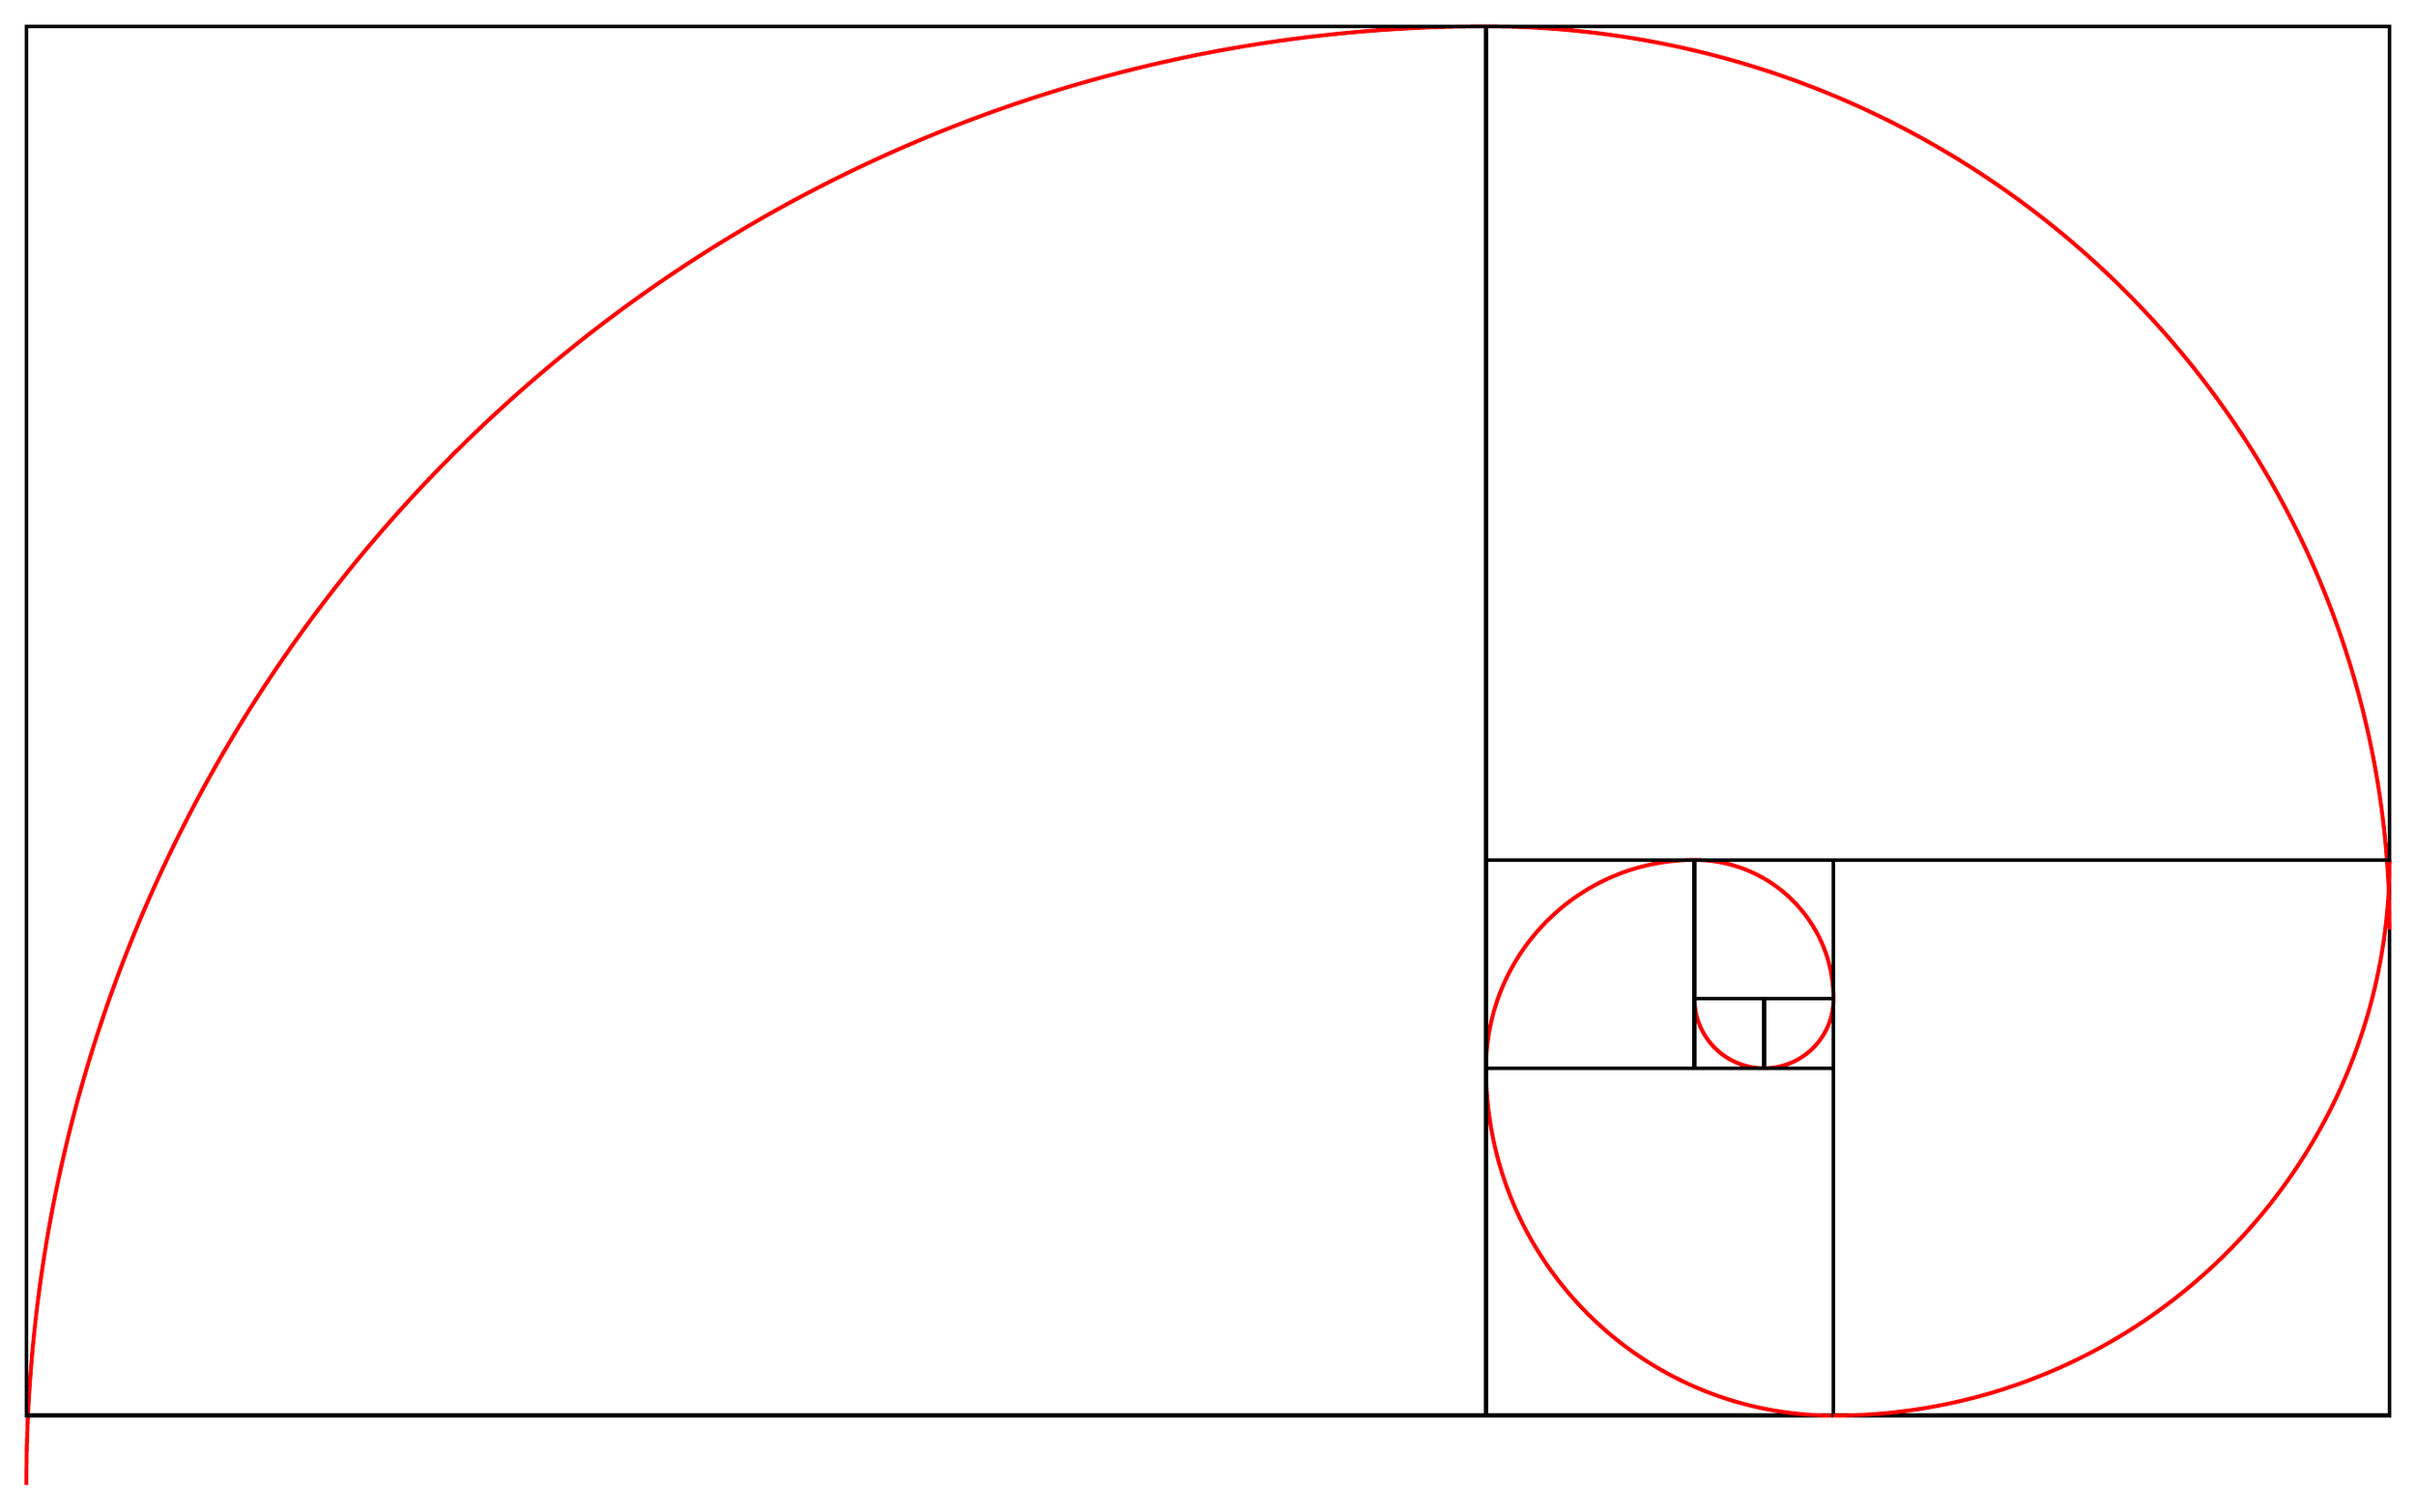
\begin{tikzpicture}[ultra thick, scale=1]
    \coordinate (Origin) at (0,0);
    \pgfmathsetmacro{\a}{1}
    \pgfmathsetmacro{\b}{1}
    \pgfmathsetmacro\c{\a+\b}
    \draw (Origin) rectangle (\a,\a);
    \draw[red] (0,\a) arc[start angle=-180, end angle=-90, radius=\a];
    \draw (\a,0) rectangle (\c,\a);
    \draw[red] (\a,0) arc[start angle=-90, end angle=0, radius=\b];
    \pgfmathsetmacro\d{\b+\c}
    \draw (\c,\a) rectangle (0,\d);
    \draw[red] (\c,\b) arc[start angle=0, end angle=90, radius=\c];
    \pgfmathsetmacro\e{\c+\d}
    \draw (0,\d) rectangle (-\d,0);
    \draw[red] (0,\d) arc[start angle=90, end angle=180, radius=\d];
    \pgfmathsetmacro\f{\d+\e}
    \draw (-\d,0) rectangle (\c,-\e);
    \draw[red] (-\d,0) arc[start angle=-180, end angle=-90, radius=\e];
    \pgfmathsetmacro\g{\e+\f}
    \draw (\c,-\e) rectangle (\c+\f,\d);
    \draw[red] (\c,-\e) arc[start angle=-90, end angle=0, radius=\f];
    \pgfmathsetmacro\h{\f+\g}
    \draw[red] (\c+\f,\c) arc[start angle=0, end angle=90, radius=\g];
    \draw (\c+\f,\d) rectangle (-\d,\c+\g);
    \pgfmathsetmacro\i{\g+\h}
    \draw[red] (-\d,\c+\g) arc[start angle=90, end angle=180, radius=\h];
    \draw (-\d,\c+\g) rectangle (-\d-\h,-\e);
\end{tikzpicture}
\end{document}
